\documentclass{magnolia}

\magtex{tex_driver={pdftex}}
\magfiche{document_nom={Fonction},
          auteur_nom={Victor Lambert},
          auteur_mail={victor.lambert@auxlazaristeslasalle.fr}}
\magexos{exos_matiere={maths},
         exos_niveau={mpsi},
         exos_chapitre_numero={3},
         exos_theme={Fonction}}
\magmisenpage{}
\maglieudiff{}
\magprocess

\begin{document}

%BEGIN_BOOK

\magsection{Fonction}

\magsubsection{Fonction}
\magsubsection{Les fonctions comme valeurs}

\exercice{nom={Dérivée numérique}}
On se donne une fonction numérique $f$ dont on souhaite obtenir une approximation de la dérivée $f'(x)$. Pour cela, on utilise les deux approximations suivantes
\[f'(x)\approx\frac{f(x+\epsilon)-f(x)}{\epsilon} \quad\text{et}\quad f'(x)\approx\frac{f(x+\epsilon)-f(x-\epsilon)}{2\epsilon}.\]
\begin{questions}
\question Écrire les fonctions \verb!derive_1(f: function, x: float, eps: float) -> float! et \verb!derive_2!, de
même signature, qui prennent en entrée $f$, $x$ et $\epsilon$ et qui renvoient respectivement l'approximation de $f'(x)$ donnée par la première et la seconde formule.
\question Testez la fonction \verb!deriv_1! avec $f(x)\defeq x^2$ puis $f(x)\defeq \ln x$ pour $x=1$ et différentes valeurs de
  $\epsilon$ de la forme $10^{-n}$. Pour quelle valeur de $n$ l'approximation est-elle la meilleure~?
% \question Étant donné une fonction $f$, observez les premières valeurs de la suite
% de terme général \[u_n=-\log_{10}\abs{\frac{\phi_n(x) - f'(x)}{f'(x)}}\] o\`u $\phi_n(x)$ est le nombre flottant renvoyé par la fonction \verb!derive_1! appelée avec $x=1$ et $\epsilon=10^{-n}$. La fonction $f'$ sera implémentée en utilisant l'expression de la dérivée de $f$. 
% Donnez la signification de $u_n$ et expliquez les variations des premiers termes de la suite $(u_n)$. Estimez, en fonction de $u\approx 10^{-16}$, la valeur de $\epsilon$ qui semble minimiser l'erreur commise en utilisant la fonction \verb!derive_1! pour obtenir une approximation de $f'(x)$.
\question Répétez l'expérience avec la fonction \verb!derive_2!. Quelle conclusion pouvez-vous en tirer~?
% \question Quelle méthode recommanderiez-vous à une personne souhaitant calculer numériquement $f'(x)$ avec la meilleure précision si on a seulement accès à une fonction calculant $f(x)$~?
\end{questions}

\magsubsection{Sortie anticipée}

\exercice{nom={Doublon}}
Écrire une fonction \verb!doublon(a)! prenant en entrée une liste \verb!a! et renvoyant \verb_True_
si \verb_a_ possède un doublon et \verb_False_ sinon. Par exemple, \verb_doublon([3, 4, 7, 3, 2])_
devra renvoyer \verb_True_ car 3 est présent deux fois dans la liste. Notre fonction devra
sortir dès qu'un doublon est trouvé.

\exercice{nom={Mêmes éléments}}
Écrire une fonction \verb!memes_elements(u: list[int], v: list[int]) -> bool! déterminant si les
listes $u$ et $v$ possèdent les mêmes éléments, peu importe l'ordre et leur nombre d'occurences.
Par exemple
\begin{center}
  \verb!memes_elements([7, 3, 5, 3], [3, 7, 5])!
\end{center}
  devra répondre \verb!True! et
\verb!memes_elements([1, 7, 2], [2, 1])! devra répondre \verb!False! car 7 est présent dans la
première liste mais pas dans la seconde.

\exercice{nom={Chaine bien parenthésée}}
On dit qu'une chaine de caractères $s$ constituée de \verb_'('_ et de \verb_')'_ est bien parenthésée lorsque
chaque parenthèse ouvrante est correctement fermée. Par exemple
\verb_"(()())"_ est bien parenthésée alors que \verb_"())("_ et \verb_"(()"_ ne le sont pas.\\

En utilisant
un compteur qui compte le nombre de parenthèses ouvrantes que l'on a vu jusqu'à présent et qui ne sont pas fermées,
écrire une fonction \verb!bien_parenthesee(s: str) -> bool! nous indiquant si la chaine caractère \verb!s!,
que l'on supposera constituée uniquement de \verb_'('_ et de \verb_')'_, est bien parenthésée.



\magsubsection{Assertion, test unitaire}
\exercice{nom={Chasse aux bugs}}
Les fonctions des questions suivantes sont buguées. Pour chaque fonction, le but est de proposer un test unitaire
qui n'est pas passé par la fonction puis de corriger le bug.
\begin{questions}
\question On définit la suite de Fibonacci par
  \[F_0\defeq 0\qsep F_1\defeq 1\qsep \text{et}\quad \forall n\in\N\qsep F_{n+2}\defeq F_{n+1}+F_n.\]
  Donner un test unitaire qui n'est pas passé par la fonction suivante devant calculer le $n$-ième terme
  de la suite de Fibonacci
\begin{pythoncode}
def fibo(n):
    """fibo(n: int) -> int"""
    a = 0
    b = 1
    for _ in range(n - 1):
        a, b = b, a + b
    return b
\end{pythoncode}
  puis corriger la fonction pour qu'elle devienne valide.
\end{questions}
\magsubsection{Sortie anticipée}

\magsection{Variable locale et globale}
\magsubsection{Variable locale}
\magsubsection{Variable globale}
\magsubsection{Composition de fonctions}

\magsection{Programmation récursive}
\magsubsection{Fonction récursive pure}



\exercice{nom={Ensemble des parties}}
On suppose les ensembles représentés par des listes non triées d'éléments deux-à-deux
distincts. Rédiger une fonction \verb!subset! qui prend en argument un ensemble et qui
renvoie l'ensemble de ses parties. Par exemple \verb!subset([1,2,3])! doit
renvoyer \verb![[], [3], [2], [2, 3], [1], [1, 3], [1, 2], [1, 2, 3]]!.

\exercice{nom={Somme dans un arbre}}
Écrire une fonction \verb!somme(t)! qui prend en paramètre une séquence imbriquée, de
profondeur et de structure quelconque, dont tous les composants élémentaires sont des nombres,
et qui calcule la somme de tous ces éléments. Par exemple
\verb!somme([[[1, 2], [3, 4, 5]], 6, [7, 8], 9])! devra renvoyer 45. Pour écrire cette
fonction on pourra utiliser la fonction \verb!isinstance(t, list)! qui permet de savoir si
$t$ est une liste.

\exercice{nom={Dénombrabilité de $\N^2$}}
On démontre que l'ensemble $\N\times\N$ est dénombrable en numérotant chaque couple $(x,y)\in\N^2$ suivant le procédé suggéré par la figure ci-dessous.
\begin{center}
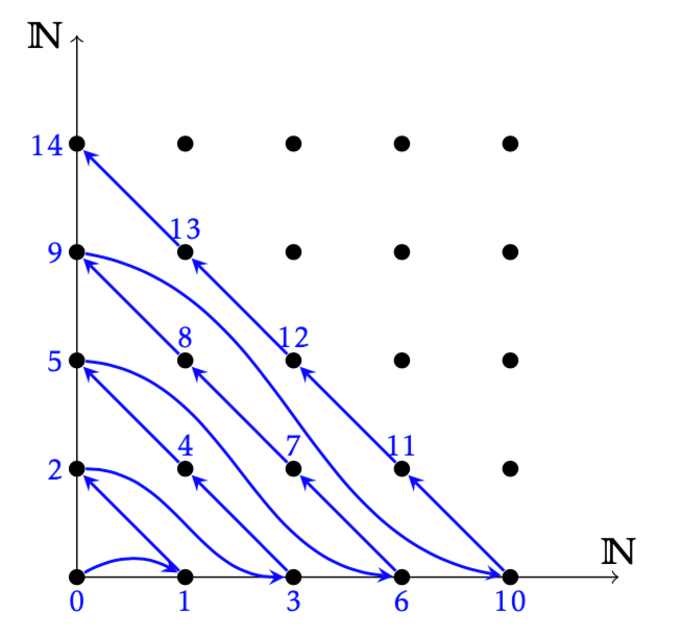
\includegraphics[width=0.3\textwidth]{../../Commun/Images/python-exos-rec-1.pdf}
\end{center}
\begin{questions}
\question Rédiger une fonction récursive qui renvoie le numéro du point de coordonnées $(x,y)\in\N^2$.
\question Rédiger la fonction réciproque, là encore, de façon récursive.
\end{questions}

\magsubsection{Fonction récursive impérative}

\exercice{nom={Triangles}}
\begin{questions}
\question Écrire une fonction récursive \verb!triangle(n)! affichant un triangle de la manière
  suivante.
\begin{pythoncode}
In [1]: triangle(5)
(*@\textcolor{purple}{*}@*)
(*@\textcolor{purple}{**}@*)
(*@\textcolor{purple}{***}@*)
(*@\textcolor{purple}{****}@*)
(*@\textcolor{purple}{*****}@*)
\end{pythoncode}
\question Écrire une fonction récursive \verb!triangle_inverse(n)! affichant un triangle de la manière
  suivante.
\begin{pythoncode}
In [2]: triangle_inverse(5)
(*@\textcolor{purple}{*****}@*)
(*@\textcolor{purple}{****}@*)
(*@\textcolor{purple}{***}@*)
(*@\textcolor{purple}{**}@*)
(*@\textcolor{purple}{*}@*)
\end{pythoncode}
\question Écrire une fonction récursive \verb!sablier(n)! affichant un demi-sablier de la manière
  suivante.
\begin{pythoncode}
In [3]: sablier(4)
(*@\textcolor{purple}{****}@*)
(*@\textcolor{purple}{***}@*)
(*@\textcolor{purple}{**}@*)
(*@\textcolor{purple}{*}@*)
(*@\textcolor{purple}{**}@*)
(*@\textcolor{purple}{***}@*)
(*@\textcolor{purple}{****}@*)
\end{pythoncode}
\end{questions}

\exercice{nom={Cercles}}
On suppose disposer d'une fonction \verb!circle([x, y], r)! qui trace à l'écran un cercle de
centre $(x,y)$ et de rayon $r$.
\begin{questions}
\question Définir une fonction récursive permettant de tracer le dessin ci-dessous où le
  cercle le plus gros est de rayon 1 de centre de coordonnées $(0,0)$ et chaque cercle est
	de rayon deux fois plus petit que celui de la génération précédente.
\begin{center}
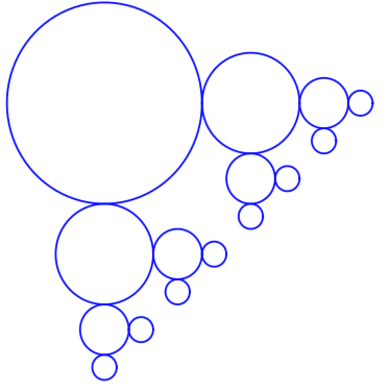
\includegraphics[width=0.2\textwidth]{../../Commun/Images/python-exos-rec-3.pdf}
\end{center}
\question Même question avec ce dessin.
\begin{center}
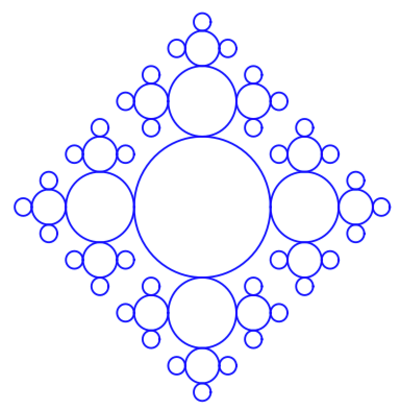
\includegraphics[width=0.2\textwidth]{../../Commun/Images/python-exos-rec-4.pdf}
\end{center}
\end{questions}

\exercice{nom={Variante sur les tours de \textsc{Hanoï}}}
Résoudre le problème des tours de Hanoï en s’imposant une contrainte supplémentaire~: tout mouvement entre les tiges 1 et 3 est interdit 

\exercice{nom={Problème des $n$ reines}}
Le problème des $n$ reines consiste à placer $n$ reines sur un échiquier de sorte que
deux reines quelconques ne puissent pas s'attaquer, c'est-à-dire qu'il ne faut pas que
deux reines partagent une même ligne, une même colonne ou une même diagonale. De telles
positions seront qualifiées dans cet exercice de \emph{valides}. Il est évident que
dans chaque colonne doit se trouver une et une seule reine. Ainsi, il est possible de
représenter ce problème par un tableau de $n$ cases $q=[q_0,\ldots,q_{n-1}]$ dans lequel
$q_j$ désigne la ligne dans laquelle est placée la reine de la colonne $j$. Par exemple,
le dessin ci-dessous représente la solution $[3, 6, 2, 7, 1, 4, 0, 5]$.
\begin{center}
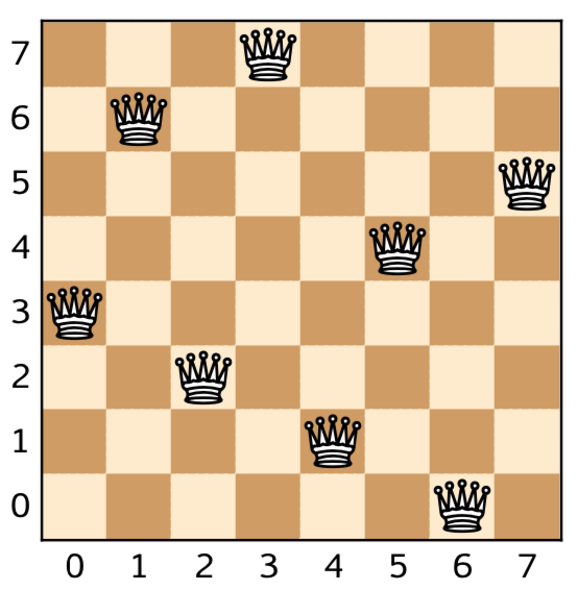
\includegraphics[width=0.3\textwidth]{../../Commun/Images/python-exos-rec-8.pdf}
\end{center}
On appellera solution partielle de rang $j$ un tableau $q$ de longueur $n$ dont les $j$
premières cases sont remplies avec des positions valides pour les reines, les
$n-j$ autres cases restant à remplir.\\

Écrire une fonction \verb!reine(q, j)! qui prend pour arguments un entier $j$ et une solution
partielle $q$ et qui réalise les opérations suivantes.
\begin{itemize}
\item Si $j=n$, cette fonction se contente d'afficher le tableau $q$. Dans ce cas, le problème
  est résolu.
\item Si $j<n$, cette fonction recherche parmi les $n$ valeurs possibles pour $q_j$ celles qui
  correspondent à des positions valides et pour chacune d'elles poursuit la recherche au
	rang $j+1$.
\end{itemize}
% \exercice{nom={Trier 3 éléments}}
% Écrire une fonction \verb!tri(a, b, c)! qui prend en argument trois nombre réels $a$, $b$ et
% $c$ et qui renvoie le triplet formé de cet 3 éléments, triés par ordre croissant.

% \exercice{nom={Parité}}
% Créer une fonction \texttt{parite} qui prend pour arguments deux entiers \texttt{x} et \texttt{y}, et qui renvoie  le booléen disant si \texttt{x} et \texttt{y}  ont même parité ou non.

	
% \exercice{nom={Triangle rectangle}}
% Créer une fonction \texttt{est\_rectangle} prenant pour argument les trois longueurs d'un triangle, et qui renvoie le booléen disant si le triangle est rectangle ou non.

	
	
% \exercice{nom={Suite récurrence}}
% Écrire une fonction \texttt{suite\_cos} qui prend pour argument un entier naturel \texttt{n} et qui affiche toutes les valeurs de $\cos(i)$ pour $i$ variant de $0$ à \texttt{n-1}.
	
% \exercice{nom={Initiales}}
% Créer une fonction \texttt{initiales} qui prend pour arguments deux chaînes de caractères \texttt{prenom} et \texttt{nom}, et qui renvoie les initiales (on suppose que les noms et prénoms ne sont pas composés...).
	
% \exercice{nom={Age et prénom}}
% Créer une fonction \texttt{age\_et\_prenom} qui prend pour argument un entier (l'âge) et une chaîne de caractères (le prénom), et qui renvoie une phrase redonnant l'âge et le nombre de lettres dans le prénom.\\ Par exemple, \texttt{age\_et\_prenom(17,'Bob')} donnera \texttt{Tu as 17 ans et ton prénom a 3 lettres.}
	
% \exercice{nom={Age}}
% Créer une fonction \texttt{age} qui prend pour argument une date de naissance (sous la forme d'une chaîne de caractère '26/11/1987'), et qui renvoie l'âge de la personne à la date d'aujourd'hui.	
% \begin{sol}
% Il y a certainement plus malin...
% \begin{pythoncode}
% def age(birth,today):
% 		jourauj,moisauj,anneeauj=int(today[0:2]),int(today[3:5]),int(today[6:10])
% 		jourbirth,moisbirth,anneebirth=int(birth[0:2]),int(birth[3:5]),int(birth[6:10])
% 		if moisauj>moisbirth:
% 				annee=anneeauj-anneebirth
% 				if jourauj>=jourbirth:
% 						mois=moisauj-moisbirth
% 				else:
% 						mois=moisauj-moisbirth-1
% 		elif moisauj==moisbirth:
% 				if jourauj>=jourbirth:
% 						annee=anneeauj-anneebirth
% 						mois=0
% 				else: 
% 						annee=anneeauj-anneebirth-1
% 						mois=11
% 		else:
% 				annee=anneeauj-anneebirth-1
% 				if jourauj>=jourbirth:
% 						mois=(moisauj-moisbirth)%12
% 				else:
% 						mois=(moisauj-moisbirth)%12-1
% 		return ("Il a "+str(annee)+" ans et "+str(mois)+" mois.")
% \end{pythoncode}
% \end{sol}

% \exercice{nom={Fonctions mystère}}
% On suppose que la variable \verb_n_ est de type \verb_int_. Donner, en fonction de $n$, la valeur et le type de l’objet renvoyé par chacune des fonctions suivantes. On ne cherchera pas à simplifier les calculs de sommes et produits mais plutôt à donner une expression utilisant des $\sum$ et des $\prod$.
% \begin{questions}
% \question
% \begin{pythoncode}
% def a(n):
% 		res = 1
% 		for i in range(1, n + 1):
% 				res = res * (i / n)
% 		return res
% \end{pythoncode}
% \question
% \begin{pythoncode}   
% def b(n):
% 		som = 0
% 		prod = 1
% 		for i in range(1, n):
% 				prod = prod * i
% 				som = som + prod
% 		return som
% \end{pythoncode}
% \question
% \begin{pythoncode}   
% def c(n):
% 		res = 0
% 		for i in range(n, 0, -1):
% 				res = res + i
% 		return res
% \end{pythoncode}
% \question
% \begin{pythoncode}    
% def d(n):
% 		q = n
% 		k = 0
% 		while q > 0:
% 				q = q // 10
% 				k = k + 1
% 		return k
% \end{pythoncode}
% \question
% \begin{pythoncode}   
% def e(n):
% 		res = 0
% 		for i in range(1, n + 1):
% 				for j in range(1, n + 1):
% 						if i > j:
% 								res = res + j
% 						else:
% 								res = res + i
% 		return res
% \end{pythoncode}
% \question
% \begin{pythoncode}    
% def f(n):
% 		u, v = 0, 2
% 		for i in range(n):
% 				u = u + v
% 				v = v + 1
% 		return u
% \end{pythoncode}
% \end{questions}


% \exercice{nom={Fonctions à compléter}}
% Complétez les programmes suivants afin qu'ils répondent aux specifications données.
% \begin{questions}
% \question
% \begin{pythoncode}
% ___

% def a(n, u0):
% 		u = ___
% 		for i in range(0, ___):
% 				u = ___
% 		return u
% \end{pythoncode}
% Cette fonction doit renvoyer le terme d'indice $n$ de la suite $(u_n)$ définie par son premier terme $u_0$ et la relation de récurrence
% \[\forall n\in\N\qsep u_{n+1}=\sqrt{u_n^2+3}.\]
% \question
% \begin{pythoncode}   
% def b(n):
% 		u = ___
% 		v = ___
% 		for i in range(___):
% 				u, v = ___
% 		return u
% \end{pythoncode}
% Cette fonction doit renvoyer le terme d'indice $n$ de la suite $(F_n)$ définie par $F_{0}=0$, $F_{1}=1$ et
% \[\forall n\in\N\qsep F_{n+2}=F_{n+1}+F_{n}.\]
% \question
% \begin{pythoncode}		
% def c(n):
% 		res = 1
% 		for i in range(1, ___):
% 				res = ___
% 				for j in range(0, ___):
% 						res= ___
% 		return res
% \end{pythoncode}
% Cette fonction doit renvoyer
% \[\sum_{i=0}^{n} \left(3^{i} +\sum_{j=1}^{n} 2i\right).\]
% \question
% \begin{pythoncode}
% def d(n):
% 		res = 0
% 		for k in range(___):
% 				p = 0
% 				for i in range(___):
% 						p = ___
% 				res = ___
% 		return res 
% \end{pythoncode}
% Cette fonction doit renvoyer
% \[\sum_{k=1}^{n} \sum_{i=1}^{k} \left(2^{i}-3ik \right).\]
% \question
% \begin{pythoncode}
% def e(n, a, b):
% 		u, v = ___
% 		i = 0
% 		while i < ___:
% 				u, v, i = ___
% 		return u, v
% \end{pythoncode}
% Cette fonction doit renvoyer le couple $(u_{n}, v_{n})$ lorsque les suites $u$ et $v$ sont définies par $u_{1}=a$, $v_{1}=b$ et 
% \[\forall n \in \N\qsep u_{n+1}=\dfrac{1}{u_{n}v_{n}} \et v_{n+1}=\dfrac{ u_{n}+v_{n}}{2}.\]
% \end{questions}

\magsubsection{Fonctions mutuellement récursives}

%END_BOOK

\end{document}
